\section{Results}

\subsection{Target trial emulation}

\begin{table}[H]
\centering
\small
\caption{Characteristics and outcomes of patients treated with thrombolysis and matched untreated controls, by time from onset to treatment. Continuous variables are shown as mean (SD); binary variables as percentages.}
\label{tab:characteristics}
\begin{tabular}{l rr rr rr}
\toprule
 & \multicolumn{2}{c}{$<$180 min} & \multicolumn{2}{c}{180--270 min} & \multicolumn{2}{c}{270--360 min} \\
\cmidrule(lr){2-3}\cmidrule(lr){4-5}\cmidrule(lr){6-7}
Characteristic & Treated & Untreated & Treated & Untreated & Treated & Untreated \\
\midrule
Number of patients & 7,378 & 7,378 & 5,512 & 5,512 & 475 & 475 \\
\addlinespace
\multicolumn{7}{l}{\textit{Baseline characteristics}} \\
\quad Age (years) & 70.5 (12.9) & 70.5 (12.9) & 70.6 (13.3) & 70.6 (13.3) & 69.3 (13.5) & 69.3 (13.5) \\
\quad Stroke severity (NIHSS) & 3.7 (1.2) & 3.7 (1.2) & 3.6 (1.2) & 3.6 (1.2) & 3.5 (1.3) & 3.5 (1.3) \\
\quad Prior disability (mRS) & 0.5 (0.9) & 0.5 (0.9) & 0.6 (1.0) & 0.6 (1.0) & 0.5 (0.8) & 0.5 (0.8) \\
\quad Hypertension (\%) & 49.9$^{**}$ & 52.4 & 53.1 & 54.9 & 50.9 & 46.3 \\
\quad Diabetes (\%) & 18.0$^{**}$ & 21.8 & 20.4 & 21.8 & 18.7 & 20.6 \\
\quad Congestive heart failure (\%) & 3.5 & 3.4 & 3.6 & 4.0 & 2.1 & 3.4 \\
\quad Atrial fibrillation (any diagnosis) (\%) & 12.2 & 12.2 & 12.1 & 12.1 & 12.6 & 12.6 \\
\quad Atrial fibrillation on anticoagulant (\%) & 2.1 & 2.1 & 2.3 & 2.3 & 3.4 & 3.4 \\
\addlinespace
\multicolumn{7}{l}{\textit{Outcomes}} \\
\quad Good outcome$^{a}$ (\%) & 78.7$^{**}$ & 71.8 & 75.8$^{**}$ & 71.3 & 77.1 & 73.7 \\
\quad Discharge disability (mRS) & 1.7 (1.3)$^{**}$ & 1.9 (1.4) & 1.8 (1.4)$^{**}$ & 1.9 (1.4) & 1.7 (1.5) & 1.8 (1.4) \\
\quad Thrombolysis-induced haemorrhage (\%) & 4.7$^{**}$ & 0.0 & 5.8$^{**}$ & 0.0 & 7.8$^{**}$ & 0.0 \\
\quad Death (\%) & 1.8 & 1.7 & 2.3 & 2.0 & 2.9 & 2.5 \\
\quad Length of stay (days) & 9.0 (18.7)$^{**}$ & 12.1 (21.1) & 10.7 (20.2)$^{**}$ & 12.6 (22.1) & 9.9 (17.6) & 11.5 (22.5) \\
\bottomrule
\end{tabular}
\par\smallskip\footnotesize mRS: modified Rankin Scale; NIHSS: National Institutes of Health Stroke Scale. $^{a}$mRS 0--2 at discharge, or discharge mRS no worse than pre-stroke mRS. Treated and matched untreated patients were compared using paired t-tests (continuous variables) and McNemar's test (binary variables): $^{*}p<0.05$; $^{**}p<0.01$. Age, stroke severity and prior disability were identical in treated and untreated patients after matching, so were not tested.
\end{table}


\begin{figure}
    \centering
    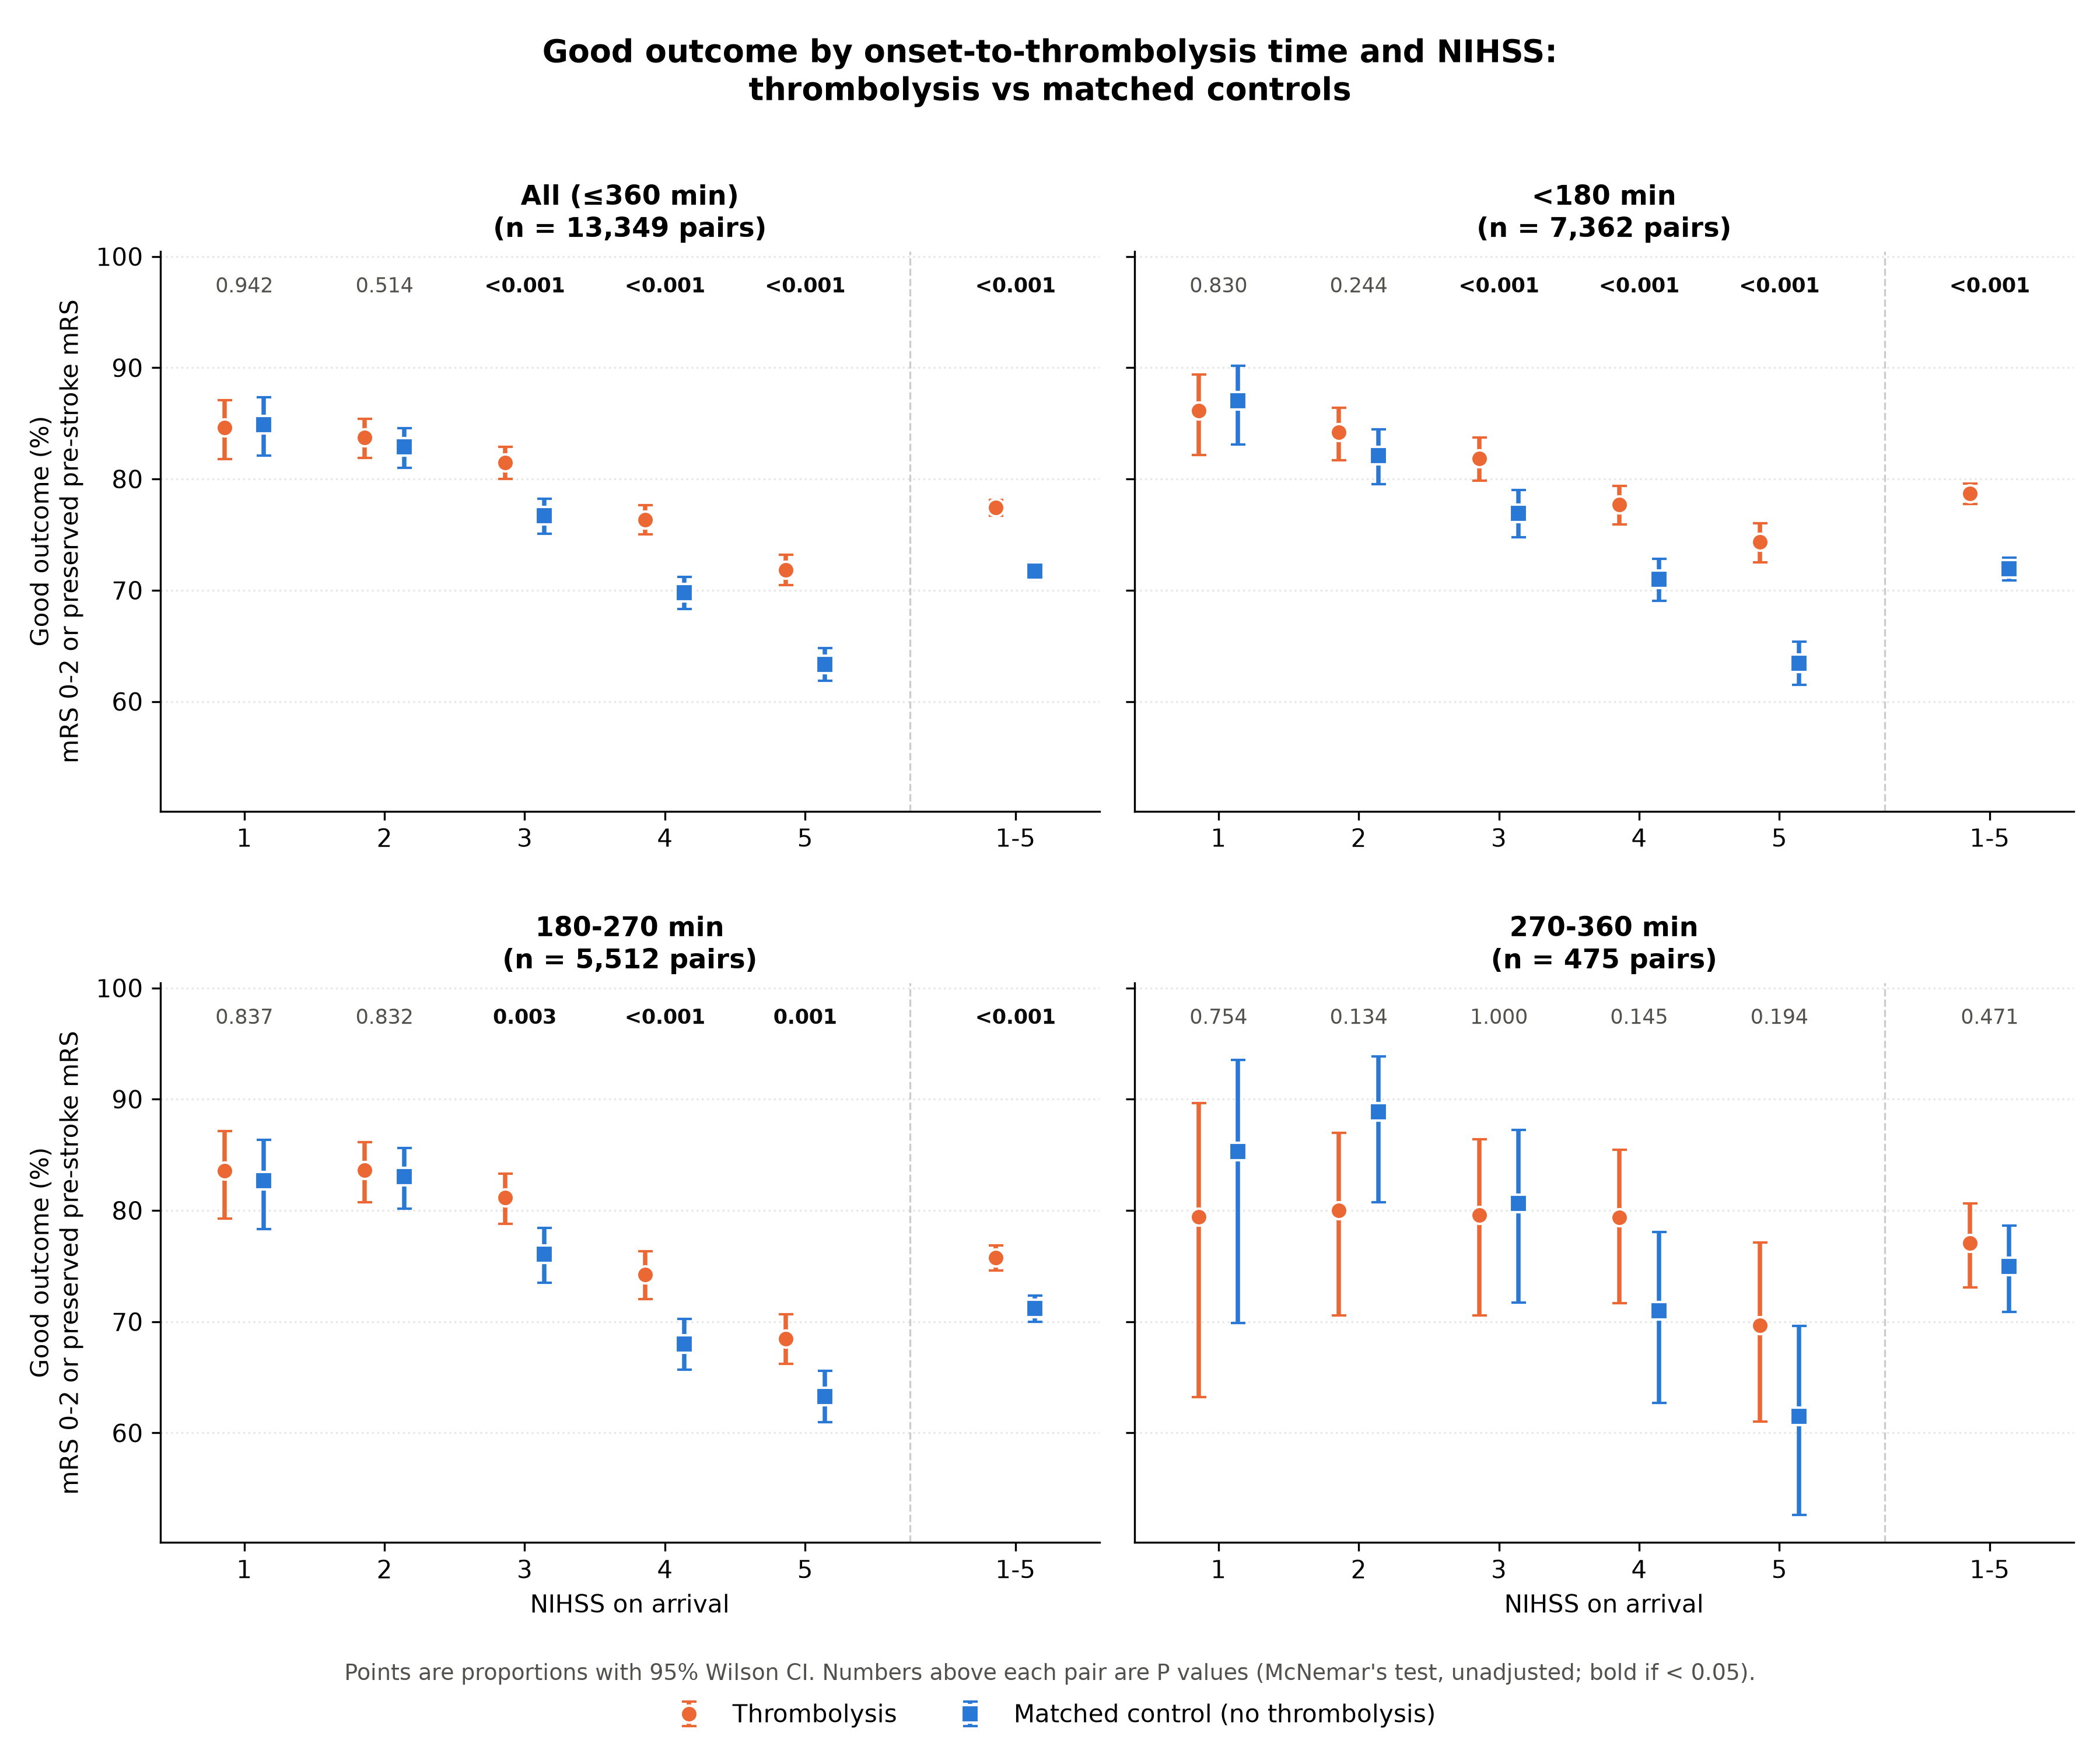
\includegraphics[width=1\linewidth]{chapters/images/mild_stroke_by_nihss_1_to_5_early_arrival_good_outcome_target_trial.png}
    \caption{Enter Caption}
    \label{fig:placeholder}
\end{figure}